\documentclass[12pt, a4paper, openany]{report}

\def\VersionRapport{1.0}

\usepackage[utf8]{inputenc} % un package
\usepackage[T1]{fontenc}      % un second package
\usepackage[francais]{babel}  % un troisième package
\usepackage{layout}
\usepackage[top=2.7cm, bottom=2.5cm, left=3.5cm, right=3cm]{geometry}
\usepackage{setspace}

\frenchbsetup{StandardLists=true} % à inclure si on utilise \usepackage[french]{babel}
\usepackage{enumitem}
\usepackage{amssymb}

\usepackage{color}
\usepackage{listings}
\definecolor{dkgreen}{rgb}{0,0.6,0}
\definecolor{gray}{rgb}{0.5,0.5,0.5}
\definecolor{mauve}{rgb}{0.58,0,0.82}

\lstset{frame=tb,
  language=Java,
  aboveskip=3mm,
  belowskip=3mm,
  showstringspaces=false,
  columns=flexible,
  basicstyle={\small\ttfamily},
  numbers=none,
  numberstyle=\tiny\color{gray},
  keywordstyle=\color{blue},
  commentstyle=\color{dkgreen},
  stringstyle=\color{mauve},
  breaklines=true,
  breakatwhitespace=true,
  tabsize=3
}

\usepackage{multirow} % pour les tableaux
\usepackage[table]{xcolor} % pour les tableaux

\usepackage{verbatim}
\usepackage{moreverb}
\usepackage{url}
\usepackage{pst-all}
\usepackage{eso-pic,graphicx}
\usepackage{caption} 
\usepackage[colorlinks=true,urlcolor=blue,linkcolor=red]{hyperref}
\usepackage{array}
\usepackage[toc,page]{appendix}
\usepackage[off]{auto-pst-pdf}
\usepackage{hyperref} % pour le sommaire table des matières
\AddThinSpaceBeforeFootnotes % à insérer si on utilise \usepackage[french]{babel}
\FrenchFootnotes % à insérer si on utilise \usepackage[french]{babel}
\usepackage{fancyhdr}
\pagestyle{headings}
\usepackage{pifont}  %pour les puces
\usepackage{amsmath} %pour les puces

\renewcommand{\appendixpagename}{Annexes}
\renewcommand{\appendixtocname}{Annexes}

\title{Theme: Rapport Performance & Robustesse}
\author{REBOUT \bsc{Mehenna}}
\author{BOUYOUCEF \bsc{Farid}}
\date{2018-2019}



%new
\newcommand{\HRule}{\rule{\linewidth}{0.5mm}}


\begin{document}

%\selectlanguage{francais}
\pagenumbering{arabic} 

\makeatletter
  \begin{titlepage}
  

  \begin{sffamily}
   \begin{center}

    % Upper part of the page. The '~' is needed because \\
    % only works if a paragraph has started.
    \includegraphics[scale=0.5]{Logo_UT3.jpg}~\\[1.5cm]

    \textsc{\LARGE Master 1 EEA ISTR/RODECO  }\\[2cm]

    \textsc{\Large Rapport Performance et Robustesse}\\[1.5cm]

    % Title
    \HRule \\[0.4cm] % saut de ligne
    { \huge \bfseries TP 1 Analyse et performances des systèmes linéaires : Asservissement d'un système à trois bacs d'eau\\[0.4cm] }

    \HRule \\[1cm]   % sous de ligne 
    \includegraphics[scale=0.1]{logomaster.jpg}
    \\[1cm]

    % Author and supervisor
    \begin{minipage}{0.4\textwidth}
      \begin{flushleft} \large
         \textsc{\emph {Réalisés par:} \\REBOUT Mehenna}\\
         \textsc{BOUYOUCEF Farid}   
          \newline
          Promotion 2018-2019 \\
      \end{flushleft}
    \end{minipage}
    \begin{minipage}{0.4\textwidth}
      \begin{flushright} \large
        \emph{Tuteur :}  \textsc{M DUROLA}\\
        \emph{Responsable de la Formation:} \textsc{M GOUAISBAUT}
      \end{flushright}
    \end{minipage}

    \vfill

    % Bottom of the page
    {\large Octobre 2018}

  \end{center}
  \end{sffamily}      
          
  \end{titlepage}
  
\makeatother



% *********************** Remerciements *****************
\chapter*{Remerciements}
 \addcontentsline{toc}{chapter}{Remerciements}

  Je tiens à exprimer ma profonde gratitude à mon promoteur, monsieur XXXX pour m'avoir encadré et guidé tout au long de l'année scolaire et mon mémoire, pour ses conseils judicieux et minutieusement prodigués.\\
  
  Aussi je tiens à lui reconnaître le temps précieux qu’il m'a consacré \\
  
   Que les membres du jury trouvent ici mes remerciements les plus vifs pour avoir accepté d’honorer par leur jugement mon travail.\\
   
   Mes sincères sentiments vont à tous ceux qui, de près ou de loin, ont contribué à la réalisation des mes études supérieurs, en particulier ma chères familles et mes amis (es).\\
   
   
%*********************** somaire **************
\renewcommand{\contentsname}{Sommaire}
\tableofcontents
%*********************** listes des figures **************
%\listoffigures
%*********************** listes des tableaux **************
%\listoftables



%*********************** INTRODUCTION **************
\chapter*{Introduction}
\addcontentsline{toc}{chapter}{Introduction}
 
  Une des raisons de construire des logiciels est pour une utilité utilisateurs.bla bla
    
    %******************* PROBLEMATIQUE**********
 \chapter*{Présentation du procédé}
\addcontentsline{toc}{chapter}{Présentation du procédé}                                                  
ina win ina thina ;;;;;;;;

	\begin{center}
    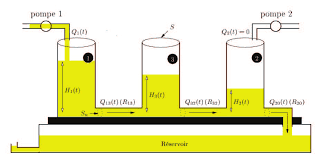
\includegraphics[scale=1]{troisBacs.png}
    \captionof{figure}{\textit{Procédé trois bacs \cite{ref1}}}
    \label{fig1}
    \end{center}


%*********************** Problématique **************
\chapter{ Analyse d'une commande proportionnelle intégrales}
 %\addcontentsline{toc}{chapter}{Analyse d'une commande proportionnelle intégrales}
 
 \section{Schéma bloc de l'asservissement}  %**** Question 1 ***** 
   % captures d’écrans 
   On donne la fonction de transfert entre le débit d'entrée  $q_{e}(p)$ et la sortie  $h_{1}(p)$ par: \\
   \begin{center}
   $G(p)=\frac {h_{1}(p)}{q_{e}(p)}=\frac{16p+20}{p^{3}+7p^{2}+12.75p+6.75}$   
   \end{center}
   
   On considère le premier correcteur de la forme : \\
   \begin{center}
   $U(p)=K\frac {1+\tau_{i}p}{\tau_{i}p}\xi(p)$ 
   \\[2cm]  
   \end{center}  
   
   \begin{center}
    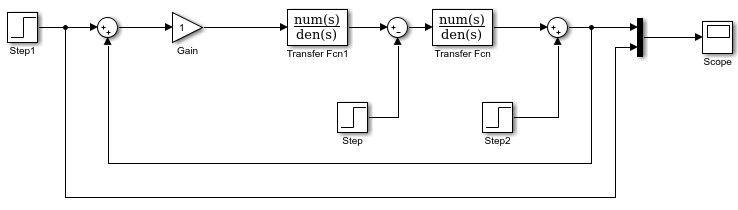
\includegraphics[scale=0.8]{schemabloc.png}
    \captionof{figure}{\textit{Schéma bloc pour un asservissement d’une commande proportionnel intégrale}}
    \label{fig2}
   \end{center}
  
   
  
 \section{Débit de fuite est constant}  %**** Question 2  *****
 
 
 On utilisant les lois de la Mécanique Des Fluides, la pression est proportionnelle au débit volumique, est on constatant que l'eau est incompressible donc le volume ne varie pas par rapport au temps, d’où le débit volumique soit constant, l'hypothèse est valable. 
 
 
 \section{Le Diagramme asymptotique de $K(p)$ }  %**** Question 3  *****
 
 On a  $G(p)=\frac {U(p)}{\xi(p)}=K\frac {1+\tau_{i}p}{\tau_{i}p}$\\
 
 est on obtient le diagramme suivant:\\
 
 ilaqagh MATLAB pour le diagramme ........
 
 
 \section{Les spécifications} %***** Question 4  *******

 D’après la première commande on a un correcteur Proportionnel Intégrale, on obtient alors un déphasage de -$\pi$ en base fréquence et aussi un gain infini, et selon le cahier de charge pour avoir une convergence vers la consigne en moins de 3 seconde, il nous faut alors une bande passante élevée, ainsi un effet intégrateur afin d'avoir une erreur de position nulle. (correcteur PI $\Rightarrow$ erreur de position nulle)
 
 
 \section{Les contraintes sur le Gabarit 1 ainsi sur le Gabarit 2}  %**** Question 5  *****
 
 Dans ces deux Gabarits, on va déterminer ses contraintes sur la fonction de sensibilité permettant de satisfaire les spécifications b) et c) de notre cahier de charge.\\[0.1cm]\\
  %%***************** Gabarit 1 *********
 \begin{itemize}[label=\ding{108},font=\small\color{black}]
\item Pour une erreur de position nulle on a:\\
$\xi_{p}= \underset{p\longrightarrow 0}{lim}\hspace{2mm} p\hspace{2mm}\xi(p)$ \\
        =$\underset{p\longrightarrow 0}{lim}\hspace{2mm} p\hspace{2mm} S(p)\hspace{2mm} r(p)$ \hspace{2cm} tel que: \hspace{0.5cm}$r(p)=\frac {1}{p}$ \\
        =$\underset{p\longrightarrow 0}{lim}\hspace{2mm} p\hspace{2mm} S(p)\hspace{2mm} \frac {1}{p} $\\ 
        =S(0)=0\\
        \\[1mm]\\
        Si on choisit $w_{1}(p)=\frac {1}{p} $ \hspace{1cm} tel que :\hspace{2mm}|$w_{1}(p).S(p)|<1$\\
        $\Rightarrow$ |$S(p)|<p$ \hspace{3mm} et on remplaçant dans la limite on obtient : \\ 
        $\xi_{p}=\underset{p\longrightarrow 0}{lim}\hspace{2mm} p\hspace{2mm} p \hspace{2mm} \frac {1}{p} $\\
        %**\\[0.2cm]
        $=\underset{p\longrightarrow 0}{lim}\hspace{2mm} p\hspace{2mm}$\\
        =\hspace{2mm}0  \\
        \\[0.5cm]\\
       $\Rightarrow$  \hspace{2mm} $|S(jw)|_{H}$<$jw$  \hspace{2mm} tel que : $|S(jw)|_{H}$ est la valeur maximum que peut atteindre le module de $S(p)$ \\
       donc : $w_{1}(p)=\frac {1}{p} $ \hspace{2mm} est un gabarit nécessaire pour une erreur de position nulle.\\
  \end{itemize}
    %*********** Gabarit 2  *******
  \begin{itemize}[label=\ding{108},font=\small\color{black}]
  \item Pour une erreur de vitesse limitée à 1 lorsque l'entrée de consigne est une rampe de pente 1 on a :\\ 
 $\xi_{v}= \underset{p\longrightarrow 0}{lim}\hspace{2mm} p\hspace{2mm}\xi(p)$ \\
    \hspace{2cm}=$\underset{p\longrightarrow 0}{lim}\hspace{2mm} p\hspace{2mm} S(p)\hspace{2mm} r(p)$ \hspace{2cm} tel que: \hspace{0.5cm}$r(p)=\frac {1}{p^{2}}$ \\
     \\[1mm]\\
        Si on choisit $w_{2}(p)=\frac {1}{p} $ \hspace{1cm} tel que :\hspace{2mm}|$w_{2}(p).S(p)|<1$\\
        $\Rightarrow$ |$S(p)|<p$ \hspace{3mm} et on remplaçant dans la limite on obtient alors : \\ 
        $\xi_{v}=\underset{p\longrightarrow 0}{lim}\hspace{2mm} p\hspace{2mm} p \hspace{2mm} \frac {1}{p^{2}} $\\
        $=\underset{p\longrightarrow 0}{lim}\hspace{2mm} \frac {p^{2}}{p^{2}}\hspace{2mm}$\\
        =\hspace{2mm}1 $\leq$1 \\
        \\[5mm]\\
        $\Rightarrow$  \hspace{2mm} $|S(jw)|_{H}$<$jw$  \hspace{2mm} tel que : $|S(jw)|_{H}$ est la valeur maximum que peut atteindre le module de $S(p)$ \\
       donc : $w_{2}(p)=\frac {1}{p} $ \hspace{2mm} est un gabarit nécessaire pour une erreur de vitesse limitée à 1 lorsque l'entrée de consigne est une rampe de pente 1.\\
  \end{itemize} 

\section{La spécification sur la vitesse de convergence ainsi le Gabarit 3 pour la sensibilité}  %**** Question 6 et 7 *****

D'après notre cahier de charge, sur le système on veut avoir une convergence vers la consigne en mois de 3 seconde, et pour que le système soit plus rapide selon la bande passante on pose alors comme une contrainte:\\
 $|T(jw)|_{db}-|T(0)|_{db} \hspace{0.2cm} > \hspace{0.2cm} 3_{db}$\\ 
 \\[0.07cm]\\
 et pour avoir une condition suffisante, alors d'après la contrainte supposée ci-dessus on a :\\
 \\[1mm]\\
 20.log($|T(jw)|_{db}-|T(0)|_{db}$) \hspace{0.2cm} > \hspace{0.2cm} 20.logS($3_{db}$)\\
 
$\Rightarrow\hspace{0.2cm} \frac {|T(jw)|}{|T(0)|} \hspace{0.2cm} > \hspace{0.2cm} 10^{3/20} \hspace{0.2cm}=1/\sqrt{2} \hspace{0.5cm} avec : \hspace{0.2cm} |T(0)|=1$ \\

$\Rightarrow\hspace{0.2cm} |T(jw)| \hspace{0.2cm} > \hspace{0.2cm} 1/\sqrt{2}$ \\

on choisit alors :$\hspace{0.3cm} |S(jw)|\hspace{0.2cm}\leq \hspace{0.2cm} 1-(1/\sqrt{2}).......(1)$ \\
 
et on a aussi: $\hspace{0.3cm} |T(jw)+S(jw)|\hspace{0.2cm}= \hspace{0.2cm} 1$\\

alors: $\hspace{0.3cm} |T(jw)|+|S(jw)|\hspace{0.2cm}\geq \hspace{0.2cm} 1........(2)$\\  

de (1) on a : $1/\sqrt{2}\leq 1-|S(jw)|........(3)$ \\

et aussi de (2) $|T(jw)|\geq 1-|S(jw)|.......(4)$ \\

alors de (3) et de (4) on obtient: \\
 
 $\hspace{0.3cm} 1/\sqrt{2}\hspace{0.2cm} \leq 1-|S(jw)| \hspace{0.2cm}\leq |T(jw)|$ \\
 
 $\Rightarrow \hspace{0.3cm} |T(jw)| \hspace{0.2cm} \geq 1/\sqrt{2}$ \\
 
donc la condition est suffisante, et cela on va calculer le module en dB de la fonction de sensibilité selon ce choit : \\

on a alors : $|S(jw)|\hspace{0.2cm}\leq 1-(1/\sqrt{2}) \hspace{0.3cm} , \forall w\in[0,w_{c}] $ \\ 

 $20.log(1-(1/\sqrt{2})\hspace{0.2cm} \simeq \hspace{0.2cm} -10.67$  \\
 
 $\Rightarrow |S(jw)|_{db}\hspace{0.2cm} \leq \hspace{0.2cm} -10.67 \hspace{0.3cm} , \forall w\in[0,w_{c}] $  \\
 
 donc : le Gabarit 3 est nécessaire pour la fonction de sensibilité quelque soit $w\in[0,w_{c}]. $   
 
 
\section{La spécification selon les oscillations (Gabarit 4)}  %**** Question 8 ***** 

selon notre cahier de charge, il est indiqué que des oscillations ne sont pas souhaitables
 
   
 



   
%*********************** Loop-shaping **************
\chapter{Réalisation d'une commande Loop-shaping}
 


% *********************** Conclusion *****************
\chapter*{Conclusion}
\addcontentsline{toc}{chapter}{Conclusion}


%Bibliographie 
\bibliographystyle{alpha}
\bibliography{biblio}
\end{document}





